
% Default to the notebook output style

    


% Inherit from the specified cell style.




    
\documentclass[11pt]{article}

    
    
    \usepackage[T1]{fontenc}
    % Nicer default font than Computer Modern for most use cases
    \usepackage{palatino}

    % Basic figure setup, for now with no caption control since it's done
    % automatically by Pandoc (which extracts ![](path) syntax from Markdown).
    \usepackage{graphicx}
    % We will generate all images so they have a width \maxwidth. This means
    % that they will get their normal width if they fit onto the page, but
    % are scaled down if they would overflow the margins.
    \makeatletter
    \def\maxwidth{\ifdim\Gin@nat@width>\linewidth\linewidth
    \else\Gin@nat@width\fi}
    \makeatother
    \let\Oldincludegraphics\includegraphics
    % Set max figure width to be 80% of text width, for now hardcoded.
    \renewcommand{\includegraphics}[1]{\Oldincludegraphics[width=.8\maxwidth]{#1}}
    % Ensure that by default, figures have no caption (until we provide a
    % proper Figure object with a Caption API and a way to capture that
    % in the conversion process - todo).
    \usepackage{caption}
    \DeclareCaptionLabelFormat{nolabel}{}
    \captionsetup{labelformat=nolabel}

    \usepackage{adjustbox} % Used to constrain images to a maximum size 
    \usepackage{xcolor} % Allow colors to be defined
    \usepackage{enumerate} % Needed for markdown enumerations to work
    \usepackage{geometry} % Used to adjust the document margins
    \usepackage{amsmath} % Equations
    \usepackage{amssymb} % Equations
    \usepackage{textcomp} % defines textquotesingle
    % Hack from http://tex.stackexchange.com/a/47451/13684:
    \AtBeginDocument{%
        \def\PYZsq{\textquotesingle}% Upright quotes in Pygmentized code
    }
    \usepackage{upquote} % Upright quotes for verbatim code
    \usepackage{eurosym} % defines \euro
    \usepackage[mathletters]{ucs} % Extended unicode (utf-8) support
    \usepackage[utf8x]{inputenc} % Allow utf-8 characters in the tex document
    \usepackage{fancyvrb} % verbatim replacement that allows latex
    \usepackage{grffile} % extends the file name processing of package graphics 
                         % to support a larger range 
    % The hyperref package gives us a pdf with properly built
    % internal navigation ('pdf bookmarks' for the table of contents,
    % internal cross-reference links, web links for URLs, etc.)
    \usepackage{hyperref}
    \usepackage{longtable} % longtable support required by pandoc >1.10
    \usepackage{booktabs}  % table support for pandoc > 1.12.2
    \usepackage[normalem]{ulem} % ulem is needed to support strikethroughs (\sout)
                                % normalem makes italics be italics, not underlines
    

    
    
    % Colors for the hyperref package
    \definecolor{urlcolor}{rgb}{0,.145,.698}
    \definecolor{linkcolor}{rgb}{.71,0.21,0.01}
    \definecolor{citecolor}{rgb}{.12,.54,.11}

    % ANSI colors
    \definecolor{ansi-black}{HTML}{3E424D}
    \definecolor{ansi-black-intense}{HTML}{282C36}
    \definecolor{ansi-red}{HTML}{E75C58}
    \definecolor{ansi-red-intense}{HTML}{B22B31}
    \definecolor{ansi-green}{HTML}{00A250}
    \definecolor{ansi-green-intense}{HTML}{007427}
    \definecolor{ansi-yellow}{HTML}{DDB62B}
    \definecolor{ansi-yellow-intense}{HTML}{B27D12}
    \definecolor{ansi-blue}{HTML}{208FFB}
    \definecolor{ansi-blue-intense}{HTML}{0065CA}
    \definecolor{ansi-magenta}{HTML}{D160C4}
    \definecolor{ansi-magenta-intense}{HTML}{A03196}
    \definecolor{ansi-cyan}{HTML}{60C6C8}
    \definecolor{ansi-cyan-intense}{HTML}{258F8F}
    \definecolor{ansi-white}{HTML}{C5C1B4}
    \definecolor{ansi-white-intense}{HTML}{A1A6B2}

    % commands and environments needed by pandoc snippets
    % extracted from the output of `pandoc -s`
    \providecommand{\tightlist}{%
      \setlength{\itemsep}{0pt}\setlength{\parskip}{0pt}}
    \DefineVerbatimEnvironment{Highlighting}{Verbatim}{commandchars=\\\{\}}
    % Add ',fontsize=\small' for more characters per line
    \newenvironment{Shaded}{}{}
    \newcommand{\KeywordTok}[1]{\textcolor[rgb]{0.00,0.44,0.13}{\textbf{{#1}}}}
    \newcommand{\DataTypeTok}[1]{\textcolor[rgb]{0.56,0.13,0.00}{{#1}}}
    \newcommand{\DecValTok}[1]{\textcolor[rgb]{0.25,0.63,0.44}{{#1}}}
    \newcommand{\BaseNTok}[1]{\textcolor[rgb]{0.25,0.63,0.44}{{#1}}}
    \newcommand{\FloatTok}[1]{\textcolor[rgb]{0.25,0.63,0.44}{{#1}}}
    \newcommand{\CharTok}[1]{\textcolor[rgb]{0.25,0.44,0.63}{{#1}}}
    \newcommand{\StringTok}[1]{\textcolor[rgb]{0.25,0.44,0.63}{{#1}}}
    \newcommand{\CommentTok}[1]{\textcolor[rgb]{0.38,0.63,0.69}{\textit{{#1}}}}
    \newcommand{\OtherTok}[1]{\textcolor[rgb]{0.00,0.44,0.13}{{#1}}}
    \newcommand{\AlertTok}[1]{\textcolor[rgb]{1.00,0.00,0.00}{\textbf{{#1}}}}
    \newcommand{\FunctionTok}[1]{\textcolor[rgb]{0.02,0.16,0.49}{{#1}}}
    \newcommand{\RegionMarkerTok}[1]{{#1}}
    \newcommand{\ErrorTok}[1]{\textcolor[rgb]{1.00,0.00,0.00}{\textbf{{#1}}}}
    \newcommand{\NormalTok}[1]{{#1}}
    
    % Additional commands for more recent versions of Pandoc
    \newcommand{\ConstantTok}[1]{\textcolor[rgb]{0.53,0.00,0.00}{{#1}}}
    \newcommand{\SpecialCharTok}[1]{\textcolor[rgb]{0.25,0.44,0.63}{{#1}}}
    \newcommand{\VerbatimStringTok}[1]{\textcolor[rgb]{0.25,0.44,0.63}{{#1}}}
    \newcommand{\SpecialStringTok}[1]{\textcolor[rgb]{0.73,0.40,0.53}{{#1}}}
    \newcommand{\ImportTok}[1]{{#1}}
    \newcommand{\DocumentationTok}[1]{\textcolor[rgb]{0.73,0.13,0.13}{\textit{{#1}}}}
    \newcommand{\AnnotationTok}[1]{\textcolor[rgb]{0.38,0.63,0.69}{\textbf{\textit{{#1}}}}}
    \newcommand{\CommentVarTok}[1]{\textcolor[rgb]{0.38,0.63,0.69}{\textbf{\textit{{#1}}}}}
    \newcommand{\VariableTok}[1]{\textcolor[rgb]{0.10,0.09,0.49}{{#1}}}
    \newcommand{\ControlFlowTok}[1]{\textcolor[rgb]{0.00,0.44,0.13}{\textbf{{#1}}}}
    \newcommand{\OperatorTok}[1]{\textcolor[rgb]{0.40,0.40,0.40}{{#1}}}
    \newcommand{\BuiltInTok}[1]{{#1}}
    \newcommand{\ExtensionTok}[1]{{#1}}
    \newcommand{\PreprocessorTok}[1]{\textcolor[rgb]{0.74,0.48,0.00}{{#1}}}
    \newcommand{\AttributeTok}[1]{\textcolor[rgb]{0.49,0.56,0.16}{{#1}}}
    \newcommand{\InformationTok}[1]{\textcolor[rgb]{0.38,0.63,0.69}{\textbf{\textit{{#1}}}}}
    \newcommand{\WarningTok}[1]{\textcolor[rgb]{0.38,0.63,0.69}{\textbf{\textit{{#1}}}}}
    
    
    % Define a nice break command that doesn't care if a line doesn't already
    % exist.
    \def\br{\hspace*{\fill} \\* }
    % Math Jax compatability definitions
    \def\gt{>}
    \def\lt{<}
    % Document parameters
    \title{eye\_report}
    
    
    

    % Pygments definitions
    
\makeatletter
\def\PY@reset{\let\PY@it=\relax \let\PY@bf=\relax%
    \let\PY@ul=\relax \let\PY@tc=\relax%
    \let\PY@bc=\relax \let\PY@ff=\relax}
\def\PY@tok#1{\csname PY@tok@#1\endcsname}
\def\PY@toks#1+{\ifx\relax#1\empty\else%
    \PY@tok{#1}\expandafter\PY@toks\fi}
\def\PY@do#1{\PY@bc{\PY@tc{\PY@ul{%
    \PY@it{\PY@bf{\PY@ff{#1}}}}}}}
\def\PY#1#2{\PY@reset\PY@toks#1+\relax+\PY@do{#2}}

\expandafter\def\csname PY@tok@gd\endcsname{\def\PY@tc##1{\textcolor[rgb]{0.63,0.00,0.00}{##1}}}
\expandafter\def\csname PY@tok@gu\endcsname{\let\PY@bf=\textbf\def\PY@tc##1{\textcolor[rgb]{0.50,0.00,0.50}{##1}}}
\expandafter\def\csname PY@tok@gt\endcsname{\def\PY@tc##1{\textcolor[rgb]{0.00,0.27,0.87}{##1}}}
\expandafter\def\csname PY@tok@gs\endcsname{\let\PY@bf=\textbf}
\expandafter\def\csname PY@tok@gr\endcsname{\def\PY@tc##1{\textcolor[rgb]{1.00,0.00,0.00}{##1}}}
\expandafter\def\csname PY@tok@cm\endcsname{\let\PY@it=\textit\def\PY@tc##1{\textcolor[rgb]{0.25,0.50,0.50}{##1}}}
\expandafter\def\csname PY@tok@vg\endcsname{\def\PY@tc##1{\textcolor[rgb]{0.10,0.09,0.49}{##1}}}
\expandafter\def\csname PY@tok@vi\endcsname{\def\PY@tc##1{\textcolor[rgb]{0.10,0.09,0.49}{##1}}}
\expandafter\def\csname PY@tok@mh\endcsname{\def\PY@tc##1{\textcolor[rgb]{0.40,0.40,0.40}{##1}}}
\expandafter\def\csname PY@tok@cs\endcsname{\let\PY@it=\textit\def\PY@tc##1{\textcolor[rgb]{0.25,0.50,0.50}{##1}}}
\expandafter\def\csname PY@tok@ge\endcsname{\let\PY@it=\textit}
\expandafter\def\csname PY@tok@vc\endcsname{\def\PY@tc##1{\textcolor[rgb]{0.10,0.09,0.49}{##1}}}
\expandafter\def\csname PY@tok@il\endcsname{\def\PY@tc##1{\textcolor[rgb]{0.40,0.40,0.40}{##1}}}
\expandafter\def\csname PY@tok@go\endcsname{\def\PY@tc##1{\textcolor[rgb]{0.53,0.53,0.53}{##1}}}
\expandafter\def\csname PY@tok@cp\endcsname{\def\PY@tc##1{\textcolor[rgb]{0.74,0.48,0.00}{##1}}}
\expandafter\def\csname PY@tok@gi\endcsname{\def\PY@tc##1{\textcolor[rgb]{0.00,0.63,0.00}{##1}}}
\expandafter\def\csname PY@tok@gh\endcsname{\let\PY@bf=\textbf\def\PY@tc##1{\textcolor[rgb]{0.00,0.00,0.50}{##1}}}
\expandafter\def\csname PY@tok@ni\endcsname{\let\PY@bf=\textbf\def\PY@tc##1{\textcolor[rgb]{0.60,0.60,0.60}{##1}}}
\expandafter\def\csname PY@tok@nl\endcsname{\def\PY@tc##1{\textcolor[rgb]{0.63,0.63,0.00}{##1}}}
\expandafter\def\csname PY@tok@nn\endcsname{\let\PY@bf=\textbf\def\PY@tc##1{\textcolor[rgb]{0.00,0.00,1.00}{##1}}}
\expandafter\def\csname PY@tok@no\endcsname{\def\PY@tc##1{\textcolor[rgb]{0.53,0.00,0.00}{##1}}}
\expandafter\def\csname PY@tok@na\endcsname{\def\PY@tc##1{\textcolor[rgb]{0.49,0.56,0.16}{##1}}}
\expandafter\def\csname PY@tok@nb\endcsname{\def\PY@tc##1{\textcolor[rgb]{0.00,0.50,0.00}{##1}}}
\expandafter\def\csname PY@tok@nc\endcsname{\let\PY@bf=\textbf\def\PY@tc##1{\textcolor[rgb]{0.00,0.00,1.00}{##1}}}
\expandafter\def\csname PY@tok@nd\endcsname{\def\PY@tc##1{\textcolor[rgb]{0.67,0.13,1.00}{##1}}}
\expandafter\def\csname PY@tok@ne\endcsname{\let\PY@bf=\textbf\def\PY@tc##1{\textcolor[rgb]{0.82,0.25,0.23}{##1}}}
\expandafter\def\csname PY@tok@nf\endcsname{\def\PY@tc##1{\textcolor[rgb]{0.00,0.00,1.00}{##1}}}
\expandafter\def\csname PY@tok@si\endcsname{\let\PY@bf=\textbf\def\PY@tc##1{\textcolor[rgb]{0.73,0.40,0.53}{##1}}}
\expandafter\def\csname PY@tok@s2\endcsname{\def\PY@tc##1{\textcolor[rgb]{0.73,0.13,0.13}{##1}}}
\expandafter\def\csname PY@tok@nt\endcsname{\let\PY@bf=\textbf\def\PY@tc##1{\textcolor[rgb]{0.00,0.50,0.00}{##1}}}
\expandafter\def\csname PY@tok@nv\endcsname{\def\PY@tc##1{\textcolor[rgb]{0.10,0.09,0.49}{##1}}}
\expandafter\def\csname PY@tok@s1\endcsname{\def\PY@tc##1{\textcolor[rgb]{0.73,0.13,0.13}{##1}}}
\expandafter\def\csname PY@tok@ch\endcsname{\let\PY@it=\textit\def\PY@tc##1{\textcolor[rgb]{0.25,0.50,0.50}{##1}}}
\expandafter\def\csname PY@tok@m\endcsname{\def\PY@tc##1{\textcolor[rgb]{0.40,0.40,0.40}{##1}}}
\expandafter\def\csname PY@tok@gp\endcsname{\let\PY@bf=\textbf\def\PY@tc##1{\textcolor[rgb]{0.00,0.00,0.50}{##1}}}
\expandafter\def\csname PY@tok@sh\endcsname{\def\PY@tc##1{\textcolor[rgb]{0.73,0.13,0.13}{##1}}}
\expandafter\def\csname PY@tok@ow\endcsname{\let\PY@bf=\textbf\def\PY@tc##1{\textcolor[rgb]{0.67,0.13,1.00}{##1}}}
\expandafter\def\csname PY@tok@sx\endcsname{\def\PY@tc##1{\textcolor[rgb]{0.00,0.50,0.00}{##1}}}
\expandafter\def\csname PY@tok@bp\endcsname{\def\PY@tc##1{\textcolor[rgb]{0.00,0.50,0.00}{##1}}}
\expandafter\def\csname PY@tok@c1\endcsname{\let\PY@it=\textit\def\PY@tc##1{\textcolor[rgb]{0.25,0.50,0.50}{##1}}}
\expandafter\def\csname PY@tok@o\endcsname{\def\PY@tc##1{\textcolor[rgb]{0.40,0.40,0.40}{##1}}}
\expandafter\def\csname PY@tok@kc\endcsname{\let\PY@bf=\textbf\def\PY@tc##1{\textcolor[rgb]{0.00,0.50,0.00}{##1}}}
\expandafter\def\csname PY@tok@c\endcsname{\let\PY@it=\textit\def\PY@tc##1{\textcolor[rgb]{0.25,0.50,0.50}{##1}}}
\expandafter\def\csname PY@tok@mf\endcsname{\def\PY@tc##1{\textcolor[rgb]{0.40,0.40,0.40}{##1}}}
\expandafter\def\csname PY@tok@err\endcsname{\def\PY@bc##1{\setlength{\fboxsep}{0pt}\fcolorbox[rgb]{1.00,0.00,0.00}{1,1,1}{\strut ##1}}}
\expandafter\def\csname PY@tok@mb\endcsname{\def\PY@tc##1{\textcolor[rgb]{0.40,0.40,0.40}{##1}}}
\expandafter\def\csname PY@tok@ss\endcsname{\def\PY@tc##1{\textcolor[rgb]{0.10,0.09,0.49}{##1}}}
\expandafter\def\csname PY@tok@sr\endcsname{\def\PY@tc##1{\textcolor[rgb]{0.73,0.40,0.53}{##1}}}
\expandafter\def\csname PY@tok@mo\endcsname{\def\PY@tc##1{\textcolor[rgb]{0.40,0.40,0.40}{##1}}}
\expandafter\def\csname PY@tok@kd\endcsname{\let\PY@bf=\textbf\def\PY@tc##1{\textcolor[rgb]{0.00,0.50,0.00}{##1}}}
\expandafter\def\csname PY@tok@mi\endcsname{\def\PY@tc##1{\textcolor[rgb]{0.40,0.40,0.40}{##1}}}
\expandafter\def\csname PY@tok@kn\endcsname{\let\PY@bf=\textbf\def\PY@tc##1{\textcolor[rgb]{0.00,0.50,0.00}{##1}}}
\expandafter\def\csname PY@tok@cpf\endcsname{\let\PY@it=\textit\def\PY@tc##1{\textcolor[rgb]{0.25,0.50,0.50}{##1}}}
\expandafter\def\csname PY@tok@kr\endcsname{\let\PY@bf=\textbf\def\PY@tc##1{\textcolor[rgb]{0.00,0.50,0.00}{##1}}}
\expandafter\def\csname PY@tok@s\endcsname{\def\PY@tc##1{\textcolor[rgb]{0.73,0.13,0.13}{##1}}}
\expandafter\def\csname PY@tok@kp\endcsname{\def\PY@tc##1{\textcolor[rgb]{0.00,0.50,0.00}{##1}}}
\expandafter\def\csname PY@tok@w\endcsname{\def\PY@tc##1{\textcolor[rgb]{0.73,0.73,0.73}{##1}}}
\expandafter\def\csname PY@tok@kt\endcsname{\def\PY@tc##1{\textcolor[rgb]{0.69,0.00,0.25}{##1}}}
\expandafter\def\csname PY@tok@sc\endcsname{\def\PY@tc##1{\textcolor[rgb]{0.73,0.13,0.13}{##1}}}
\expandafter\def\csname PY@tok@sb\endcsname{\def\PY@tc##1{\textcolor[rgb]{0.73,0.13,0.13}{##1}}}
\expandafter\def\csname PY@tok@k\endcsname{\let\PY@bf=\textbf\def\PY@tc##1{\textcolor[rgb]{0.00,0.50,0.00}{##1}}}
\expandafter\def\csname PY@tok@se\endcsname{\let\PY@bf=\textbf\def\PY@tc##1{\textcolor[rgb]{0.73,0.40,0.13}{##1}}}
\expandafter\def\csname PY@tok@sd\endcsname{\let\PY@it=\textit\def\PY@tc##1{\textcolor[rgb]{0.73,0.13,0.13}{##1}}}

\def\PYZbs{\char`\\}
\def\PYZus{\char`\_}
\def\PYZob{\char`\{}
\def\PYZcb{\char`\}}
\def\PYZca{\char`\^}
\def\PYZam{\char`\&}
\def\PYZlt{\char`\<}
\def\PYZgt{\char`\>}
\def\PYZsh{\char`\#}
\def\PYZpc{\char`\%}
\def\PYZdl{\char`\$}
\def\PYZhy{\char`\-}
\def\PYZsq{\char`\'}
\def\PYZdq{\char`\"}
\def\PYZti{\char`\~}
% for compatibility with earlier versions
\def\PYZat{@}
\def\PYZlb{[}
\def\PYZrb{]}
\makeatother


    % Exact colors from NB
    \definecolor{incolor}{rgb}{0.0, 0.0, 0.5}
    \definecolor{outcolor}{rgb}{0.545, 0.0, 0.0}



    
    % Prevent overflowing lines due to hard-to-break entities
    \sloppy 
    % Setup hyperref package
    \hypersetup{
      breaklinks=true,  % so long urls are correctly broken across lines
      colorlinks=true,
      urlcolor=urlcolor,
      linkcolor=linkcolor,
      citecolor=citecolor,
      }
    % Slightly bigger margins than the latex defaults
    
    \geometry{verbose,tmargin=1in,bmargin=1in,lmargin=1in,rmargin=1in}
    
    

    \begin{document}
    
    
    \maketitle
    
    

    
    \section{Summary Report for Eye
Projects}\label{summary-report-for-eye-projects}

Darvin Yi (darvinyi{[}at{]}Stanford{[}dot{]}edu) Carson Lam
(carsonl{[}at{]}Stanford{[}dot{]}edu)

We can give the summary reports for the following projects: - Data
Preprocessing - Exudate/Microaneurysm Segmentation - Diabetic
Retinopathy Classification - Sliding Window Abnormality Detection

    \section{Data Preprocessing}\label{data-preprocessing}

We do a few things, but we'll focus on showing off the following: -
Tight Cropping - Adaptive Histogram Equalization

    \subsection{Tight Cropping}\label{tight-cropping}

Most of the image will be black background. Thus, we want to crop very
tightly around the eye as much as possible to give the network the most
information as possible.

    \begin{Verbatim}[commandchars=\\\{\}]
{\color{incolor}In [{\color{incolor}1}]:} \PY{k+kn}{import} \PY{n+nn}{numpy} \PY{k+kn}{as} \PY{n+nn}{np}
        \PY{k+kn}{import} \PY{n+nn}{scipy.misc}
        \PY{k+kn}{from} \PY{n+nn}{skimage.filters} \PY{k+kn}{import} \PY{n}{threshold\PYZus{}otsu}
        \PY{k+kn}{from} \PY{n+nn}{skimage} \PY{k+kn}{import} \PY{n}{measure}\PY{p}{,}\PY{n}{exposure}
        
        \PY{k+kn}{import} \PY{n+nn}{matplotlib.pyplot} \PY{k+kn}{as} \PY{n+nn}{plt}
        \PY{o}{\PYZpc{}}\PY{k}{matplotlib} inline
        
        \PY{c+c1}{\PYZsh{} Function to do cropping}
        \PY{k}{def} \PY{n+nf}{tight\PYZus{}crop}\PY{p}{(}\PY{n}{img}\PY{p}{,}\PY{n}{size}\PY{o}{=}\PY{n+nb+bp}{None}\PY{p}{)}\PY{p}{:}
            \PY{n}{img\PYZus{}gray} \PY{o}{=} \PY{n}{np}\PY{o}{.}\PY{n}{mean}\PY{p}{(}\PY{n}{img}\PY{p}{,} \PY{l+m+mi}{2}\PY{p}{)}
            \PY{n}{img\PYZus{}bw} \PY{o}{=} \PY{n}{img\PYZus{}gray} \PY{o}{\PYZgt{}} \PY{n}{threshold\PYZus{}otsu}\PY{p}{(}\PY{n}{img\PYZus{}gray}\PY{p}{)}
            \PY{n}{img\PYZus{}label} \PY{o}{=} \PY{n}{measure}\PY{o}{.}\PY{n}{label}\PY{p}{(}\PY{n}{img\PYZus{}bw}\PY{p}{,} \PY{n}{background}\PY{o}{=}\PY{l+m+mi}{0}\PY{p}{)}
            \PY{n}{largest\PYZus{}label} \PY{o}{=} \PY{n}{np}\PY{o}{.}\PY{n}{argmax}\PY{p}{(}\PY{n}{np}\PY{o}{.}\PY{n}{bincount}\PY{p}{(}\PY{n}{img\PYZus{}label}\PY{o}{.}\PY{n}{flatten}\PY{p}{(}\PY{p}{)}\PY{p}{)}\PY{p}{[}\PY{l+m+mi}{1}\PY{p}{:}\PY{p}{]}\PY{p}{)} \PY{o}{+} \PY{l+m+mi}{1}
            \PY{n}{img\PYZus{}circ} \PY{o}{=} \PY{p}{(}\PY{n}{img\PYZus{}label} \PY{o}{==} \PY{n}{largest\PYZus{}label}\PY{p}{)}
            \PY{n}{img\PYZus{}xs} \PY{o}{=} \PY{n}{np}\PY{o}{.}\PY{n}{sum}\PY{p}{(}\PY{n}{img\PYZus{}circ}\PY{p}{,} \PY{l+m+mi}{0}\PY{p}{)}
            \PY{n}{img\PYZus{}ys} \PY{o}{=} \PY{n}{np}\PY{o}{.}\PY{n}{sum}\PY{p}{(}\PY{n}{img\PYZus{}circ}\PY{p}{,} \PY{l+m+mi}{1}\PY{p}{)}
            \PY{n}{xs} \PY{o}{=} \PY{n}{np}\PY{o}{.}\PY{n}{where}\PY{p}{(}\PY{n}{img\PYZus{}xs} \PY{o}{\PYZgt{}} \PY{l+m+mi}{0}\PY{p}{)}
            \PY{n}{ys} \PY{o}{=} \PY{n}{np}\PY{o}{.}\PY{n}{where}\PY{p}{(}\PY{n}{img\PYZus{}ys} \PY{o}{\PYZgt{}} \PY{l+m+mi}{0}\PY{p}{)}
            \PY{n}{y\PYZus{}lo} \PY{o}{=} \PY{n}{np}\PY{o}{.}\PY{n}{min}\PY{p}{(}\PY{n}{ys}\PY{p}{)}
            \PY{n}{y\PYZus{}hi} \PY{o}{=} \PY{n}{np}\PY{o}{.}\PY{n}{max}\PY{p}{(}\PY{n}{ys}\PY{p}{)}
            \PY{n}{x\PYZus{}lo} \PY{o}{=} \PY{n}{np}\PY{o}{.}\PY{n}{min}\PY{p}{(}\PY{n}{xs}\PY{p}{)}
            \PY{n}{x\PYZus{}hi} \PY{o}{=} \PY{n}{np}\PY{o}{.}\PY{n}{max}\PY{p}{(}\PY{n}{xs}\PY{p}{)}
            \PY{n}{img\PYZus{}crop} \PY{o}{=} \PY{n}{img}\PY{p}{[}\PY{n}{y\PYZus{}lo}\PY{p}{:}\PY{n}{y\PYZus{}hi}\PY{p}{,} \PY{n}{x\PYZus{}lo}\PY{p}{:}\PY{n}{x\PYZus{}hi}\PY{p}{,} \PY{p}{:}\PY{p}{]}
            \PY{k}{return} \PY{n}{img\PYZus{}crop}
\end{Verbatim}

    \begin{Verbatim}[commandchars=\\\{\}]
{\color{incolor}In [{\color{incolor}2}]:} \PY{c+c1}{\PYZsh{} Filepath}
        \PY{n}{path\PYZus{}img} \PY{o}{=} \PY{l+s+s2}{\PYZdq{}}\PY{l+s+s2}{figures/examples/C0021833.jpg}\PY{l+s+s2}{\PYZdq{}}
        
        \PY{c+c1}{\PYZsh{} Reading in Image}
        \PY{n}{img} \PY{o}{=} \PY{n}{scipy}\PY{o}{.}\PY{n}{misc}\PY{o}{.}\PY{n}{imread}\PY{p}{(}\PY{n}{path\PYZus{}img}\PY{p}{)}
        \PY{n}{img} \PY{o}{=} \PY{n}{img}\PY{o}{.}\PY{n}{astype}\PY{p}{(}\PY{n}{np}\PY{o}{.}\PY{n}{float32}\PY{p}{)}
        \PY{n}{img} \PY{o}{/}\PY{o}{=} \PY{l+m+mi}{255}
        
        \PY{c+c1}{\PYZsh{} Cropping Image}
        \PY{n}{img\PYZus{}crop} \PY{o}{=} \PY{n}{tight\PYZus{}crop}\PY{p}{(}\PY{n}{img}\PY{p}{)}
        
        \PY{c+c1}{\PYZsh{} Plotting}
        \PY{n}{plt}\PY{o}{.}\PY{n}{rcParams}\PY{p}{[}\PY{l+s+s1}{\PYZsq{}}\PY{l+s+s1}{figure.figsize}\PY{l+s+s1}{\PYZsq{}}\PY{p}{]} \PY{o}{=} \PY{p}{[}\PY{l+m+mi}{18}\PY{p}{,}\PY{l+m+mi}{12}\PY{p}{]}
        \PY{n}{fig}\PY{p}{,}\PY{n}{ax} \PY{o}{=} \PY{n}{plt}\PY{o}{.}\PY{n}{subplots}\PY{p}{(}\PY{l+m+mi}{1}\PY{p}{,}\PY{l+m+mi}{2}\PY{p}{)}
        \PY{n}{ax}\PY{p}{[}\PY{l+m+mi}{0}\PY{p}{]}\PY{o}{.}\PY{n}{imshow}\PY{p}{(}\PY{n}{img}\PY{p}{)}
        \PY{n}{ax}\PY{p}{[}\PY{l+m+mi}{0}\PY{p}{]}\PY{o}{.}\PY{n}{axis}\PY{p}{(}\PY{l+s+s1}{\PYZsq{}}\PY{l+s+s1}{off}\PY{l+s+s1}{\PYZsq{}}\PY{p}{)}
        \PY{n}{ax}\PY{p}{[}\PY{l+m+mi}{0}\PY{p}{]}\PY{o}{.}\PY{n}{set\PYZus{}title}\PY{p}{(}\PY{l+s+s1}{\PYZsq{}}\PY{l+s+s1}{Original}\PY{l+s+s1}{\PYZsq{}}\PY{p}{)}
        \PY{n}{ax}\PY{p}{[}\PY{l+m+mi}{1}\PY{p}{]}\PY{o}{.}\PY{n}{imshow}\PY{p}{(}\PY{n}{img\PYZus{}crop}\PY{p}{)}
        \PY{n}{ax}\PY{p}{[}\PY{l+m+mi}{1}\PY{p}{]}\PY{o}{.}\PY{n}{axis}\PY{p}{(}\PY{l+s+s1}{\PYZsq{}}\PY{l+s+s1}{off}\PY{l+s+s1}{\PYZsq{}}\PY{p}{)}
        \PY{n}{ax}\PY{p}{[}\PY{l+m+mi}{1}\PY{p}{]}\PY{o}{.}\PY{n}{set\PYZus{}title}\PY{p}{(}\PY{l+s+s1}{\PYZsq{}}\PY{l+s+s1}{Tight Crop}\PY{l+s+s1}{\PYZsq{}}\PY{p}{)}
\end{Verbatim}

            \begin{Verbatim}[commandchars=\\\{\}]
{\color{outcolor}Out[{\color{outcolor}2}]:} <matplotlib.text.Text at 0xa9933c8>
\end{Verbatim}
        
    \begin{center}
    \adjustimage{max size={0.9\linewidth}{0.9\paperheight}}{eye_report_files/eye_report_4_1.png}
    \end{center}
    { \hspace*{\fill} \\}
    
    \subsection{Adaptive Histogram
Equalization}\label{adaptive-histogram-equalization}

Basically, working with 8-bit images where the signal is quite subtle,
we chose to put each channel through an adaptive histogram equalization
to make sure interesting features were not lost.

    \begin{Verbatim}[commandchars=\\\{\}]
{\color{incolor}In [{\color{incolor}3}]:} \PY{c+c1}{\PYZsh{} Function for AHE}
        \PY{k}{def} \PY{n+nf}{channelwise\PYZus{}ahe}\PY{p}{(}\PY{n}{img}\PY{p}{)}\PY{p}{:}
            \PY{n}{img\PYZus{}ahe} \PY{o}{=} \PY{n}{img}\PY{o}{.}\PY{n}{copy}\PY{p}{(}\PY{p}{)}
            \PY{k}{for} \PY{n}{i} \PY{o+ow}{in} \PY{n+nb}{range}\PY{p}{(}\PY{n}{img}\PY{o}{.}\PY{n}{shape}\PY{p}{[}\PY{l+m+mi}{2}\PY{p}{]}\PY{p}{)}\PY{p}{:}
                \PY{n}{img\PYZus{}ahe}\PY{p}{[}\PY{p}{:}\PY{p}{,}\PY{p}{:}\PY{p}{,}\PY{n}{i}\PY{p}{]} \PY{o}{=} \PY{n}{exposure}\PY{o}{.}\PY{n}{equalize\PYZus{}adapthist}\PY{p}{(}\PY{n}{img}\PY{p}{[}\PY{p}{:}\PY{p}{,}\PY{p}{:}\PY{p}{,}\PY{n}{i}\PY{p}{]}\PY{p}{,} \PY{n}{clip\PYZus{}limit}\PY{o}{=}\PY{l+m+mf}{0.03}\PY{p}{)}
            \PY{k}{return} \PY{n}{img\PYZus{}ahe}
\end{Verbatim}

    \begin{Verbatim}[commandchars=\\\{\}]
{\color{incolor}In [{\color{incolor}4}]:} \PY{c+c1}{\PYZsh{} Do Contrast Enhancement}
        \PY{n}{img\PYZus{}ahe} \PY{o}{=} \PY{n}{channelwise\PYZus{}ahe}\PY{p}{(}\PY{n}{img\PYZus{}crop}\PY{p}{)}
        
        \PY{c+c1}{\PYZsh{} Plotting}
        \PY{n}{plt}\PY{o}{.}\PY{n}{rcParams}\PY{p}{[}\PY{l+s+s1}{\PYZsq{}}\PY{l+s+s1}{figure.figsize}\PY{l+s+s1}{\PYZsq{}}\PY{p}{]} \PY{o}{=} \PY{p}{[}\PY{l+m+mi}{18}\PY{p}{,}\PY{l+m+mi}{12}\PY{p}{]}
        \PY{n}{fig}\PY{p}{,}\PY{n}{ax} \PY{o}{=} \PY{n}{plt}\PY{o}{.}\PY{n}{subplots}\PY{p}{(}\PY{l+m+mi}{1}\PY{p}{,}\PY{l+m+mi}{2}\PY{p}{)}
        \PY{n}{ax}\PY{p}{[}\PY{l+m+mi}{0}\PY{p}{]}\PY{o}{.}\PY{n}{imshow}\PY{p}{(}\PY{n}{img\PYZus{}crop}\PY{p}{)}
        \PY{n}{ax}\PY{p}{[}\PY{l+m+mi}{0}\PY{p}{]}\PY{o}{.}\PY{n}{axis}\PY{p}{(}\PY{l+s+s1}{\PYZsq{}}\PY{l+s+s1}{off}\PY{l+s+s1}{\PYZsq{}}\PY{p}{)}
        \PY{n}{ax}\PY{p}{[}\PY{l+m+mi}{0}\PY{p}{]}\PY{o}{.}\PY{n}{set\PYZus{}title}\PY{p}{(}\PY{l+s+s1}{\PYZsq{}}\PY{l+s+s1}{Original}\PY{l+s+s1}{\PYZsq{}}\PY{p}{)}
        \PY{n}{ax}\PY{p}{[}\PY{l+m+mi}{1}\PY{p}{]}\PY{o}{.}\PY{n}{imshow}\PY{p}{(}\PY{n}{img\PYZus{}ahe}\PY{p}{)}
        \PY{n}{ax}\PY{p}{[}\PY{l+m+mi}{1}\PY{p}{]}\PY{o}{.}\PY{n}{axis}\PY{p}{(}\PY{l+s+s1}{\PYZsq{}}\PY{l+s+s1}{off}\PY{l+s+s1}{\PYZsq{}}\PY{p}{)}
        \PY{n}{ax}\PY{p}{[}\PY{l+m+mi}{1}\PY{p}{]}\PY{o}{.}\PY{n}{set\PYZus{}title}\PY{p}{(}\PY{l+s+s1}{\PYZsq{}}\PY{l+s+s1}{High Contrast}\PY{l+s+s1}{\PYZsq{}}\PY{p}{)}
\end{Verbatim}

    \begin{Verbatim}[commandchars=\\\{\}]
C:\textbackslash{}Users\textbackslash{}yidar\textbackslash{}AppData\textbackslash{}Local\textbackslash{}Continuum\textbackslash{}Anaconda2\textbackslash{}lib\textbackslash{}site-packages\textbackslash{}skimage\textbackslash{}util\textbackslash{}dtype.py:110: UserWarning: Possible precision loss when converting from float32 to uint16
  "\%s to \%s" \% (dtypeobj\_in, dtypeobj))

    \end{Verbatim}

            \begin{Verbatim}[commandchars=\\\{\}]
{\color{outcolor}Out[{\color{outcolor}4}]:} <matplotlib.text.Text at 0xa681710>
\end{Verbatim}
        
    \begin{center}
    \adjustimage{max size={0.9\linewidth}{0.9\paperheight}}{eye_report_files/eye_report_7_2.png}
    \end{center}
    { \hspace*{\fill} \\}
    
    To see why this contrast enhancement is helpful, we can look at
microaneurysms.

    \begin{Verbatim}[commandchars=\\\{\}]
{\color{incolor}In [{\color{incolor}5}]:} \PY{n}{img\PYZus{}MA} \PY{o}{=} \PY{n}{img\PYZus{}crop}\PY{p}{[}\PY{l+m+mi}{825}\PY{p}{:}\PY{l+m+mi}{925}\PY{p}{,}\PY{l+m+mi}{250}\PY{p}{:}\PY{l+m+mi}{450}\PY{p}{,}\PY{p}{:}\PY{p}{]}
        \PY{n}{img\PYZus{}MA\PYZus{}ahe} \PY{o}{=} \PY{n}{img\PYZus{}ahe}\PY{p}{[}\PY{l+m+mi}{825}\PY{p}{:}\PY{l+m+mi}{925}\PY{p}{,}\PY{l+m+mi}{250}\PY{p}{:}\PY{l+m+mi}{450}\PY{p}{,}\PY{p}{:}\PY{p}{]}
        
        \PY{c+c1}{\PYZsh{} Plotting}
        \PY{n}{plt}\PY{o}{.}\PY{n}{rcParams}\PY{p}{[}\PY{l+s+s1}{\PYZsq{}}\PY{l+s+s1}{figure.figsize}\PY{l+s+s1}{\PYZsq{}}\PY{p}{]} \PY{o}{=} \PY{p}{[}\PY{l+m+mi}{18}\PY{p}{,}\PY{l+m+mi}{12}\PY{p}{]}
        \PY{n}{fig}\PY{p}{,}\PY{n}{ax} \PY{o}{=} \PY{n}{plt}\PY{o}{.}\PY{n}{subplots}\PY{p}{(}\PY{l+m+mi}{1}\PY{p}{,}\PY{l+m+mi}{2}\PY{p}{)}
        \PY{n}{ax}\PY{p}{[}\PY{l+m+mi}{0}\PY{p}{]}\PY{o}{.}\PY{n}{imshow}\PY{p}{(}\PY{n}{img\PYZus{}MA}\PY{p}{)}
        \PY{n}{ax}\PY{p}{[}\PY{l+m+mi}{0}\PY{p}{]}\PY{o}{.}\PY{n}{axis}\PY{p}{(}\PY{l+s+s1}{\PYZsq{}}\PY{l+s+s1}{off}\PY{l+s+s1}{\PYZsq{}}\PY{p}{)}
        \PY{n}{ax}\PY{p}{[}\PY{l+m+mi}{0}\PY{p}{]}\PY{o}{.}\PY{n}{set\PYZus{}title}\PY{p}{(}\PY{l+s+s1}{\PYZsq{}}\PY{l+s+s1}{Original}\PY{l+s+s1}{\PYZsq{}}\PY{p}{)}
        \PY{n}{ax}\PY{p}{[}\PY{l+m+mi}{1}\PY{p}{]}\PY{o}{.}\PY{n}{imshow}\PY{p}{(}\PY{n}{img\PYZus{}MA\PYZus{}ahe}\PY{p}{)}
        \PY{n}{ax}\PY{p}{[}\PY{l+m+mi}{1}\PY{p}{]}\PY{o}{.}\PY{n}{axis}\PY{p}{(}\PY{l+s+s1}{\PYZsq{}}\PY{l+s+s1}{off}\PY{l+s+s1}{\PYZsq{}}\PY{p}{)}
        \PY{n}{ax}\PY{p}{[}\PY{l+m+mi}{1}\PY{p}{]}\PY{o}{.}\PY{n}{set\PYZus{}title}\PY{p}{(}\PY{l+s+s1}{\PYZsq{}}\PY{l+s+s1}{High Contrast}\PY{l+s+s1}{\PYZsq{}}\PY{p}{)}
\end{Verbatim}

            \begin{Verbatim}[commandchars=\\\{\}]
{\color{outcolor}Out[{\color{outcolor}5}]:} <matplotlib.text.Text at 0xa882320>
\end{Verbatim}
        
    \begin{center}
    \adjustimage{max size={0.9\linewidth}{0.9\paperheight}}{eye_report_files/eye_report_9_1.png}
    \end{center}
    { \hspace*{\fill} \\}
    
    Even zoomed in, it's hard to tell the microaneurysms in the original
image. However, in the high contrast image, it's a little easier. Easier
for the human will most likely be easier for the machine.

    \subsection{Exudate/Microaneurysm
Segmentation}\label{exudatemicroaneurysm-segmentation}

\subsubsection{Data: A Color Fundus Image
Database}\label{data-a-color-fundus-image-database}

The data comes from a French group called
\href{http://www.adcis.net/en/Download-Third-Party/E-Ophtha.html}{ADCIS}.
They apparently work on biomedical image analysis.

The main data that we have to work with has the following images: - 34
Patients with Exudates labeled as binary mask - 67 Patients with
Microaneurysms labeled as binary mask - 100+ Normal Patients

    \subsubsection{Preliminary work}\label{preliminary-work}

    We simply follow a simply architecture set up like the one shown by
\href{https://people.eecs.berkeley.edu/~jonlong/long_shelhamer_fcn.pdf}{Long
\emph{et. al.}}. We just put a few \texttt{conv2d\_tranpose} layers on
the end of
\href{http://www.cv-foundation.org/openaccess/content_cvpr_2015/papers/Szegedy_Going_Deeper_With_2015_CVPR_paper.pdf}{GoogLe
Net} and we already get good results.

    \subsubsection{Exudates}\label{exudates}

Even with 34 patients and less than 1 hr training on a single gpu using
default network parameters, we can segment out exudates pretty well.
Here are some examples from the validation set (i.e.~never touched by
training algorithm). Care was also taken to make sure
training/validation sets were separated by patient.

Every image below is formatted the same way. - The left image is a
grayscaled version of the original image. - The right image is the
original image overlayed with the grount truth segmentation (red=1,
blue=0) - The middle image is the original image overlayed with our
predicted softmax probability values represented by the jet-colormap
going from colder blue colors for less probable and hotter red colors
for more probable of being a pixel of interest.

\begin{figure}
\centering
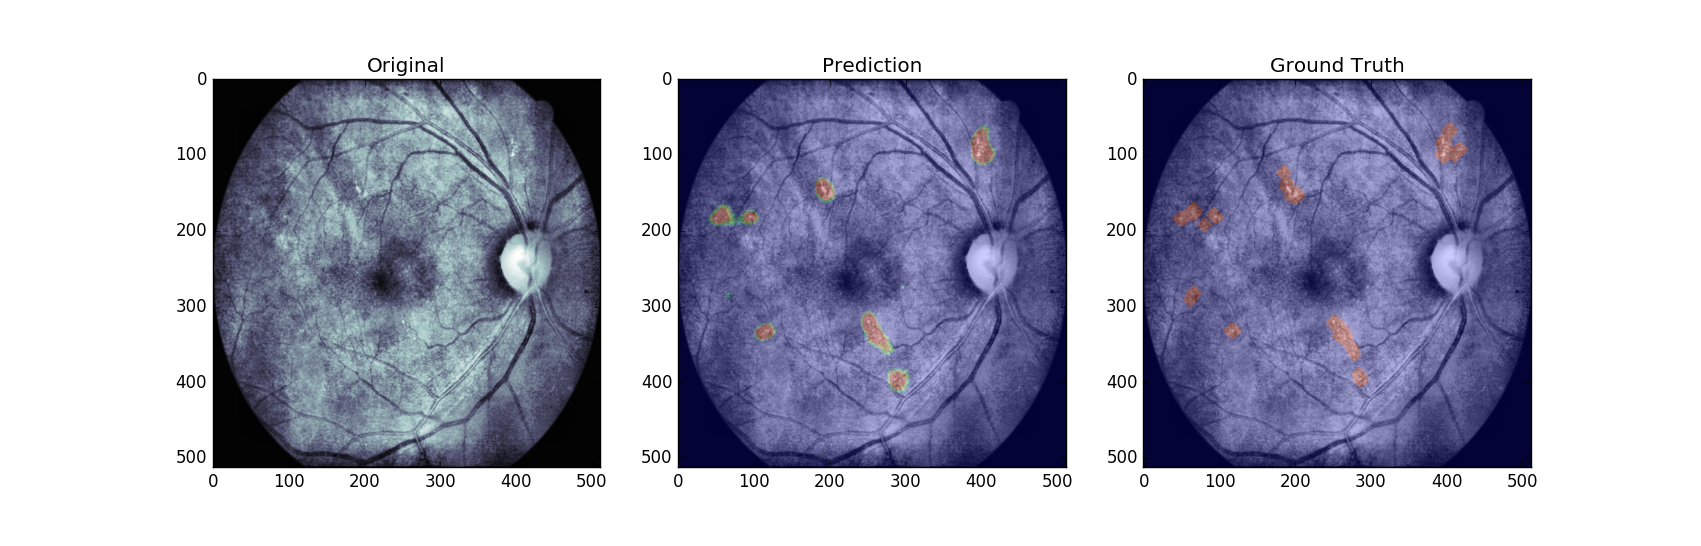
\includegraphics{C:/Users/yidar/Desktop/candle/reports/figures/EX-seg/C0021833.h5.png}
\caption{}
\end{figure}

\begin{figure}
\centering
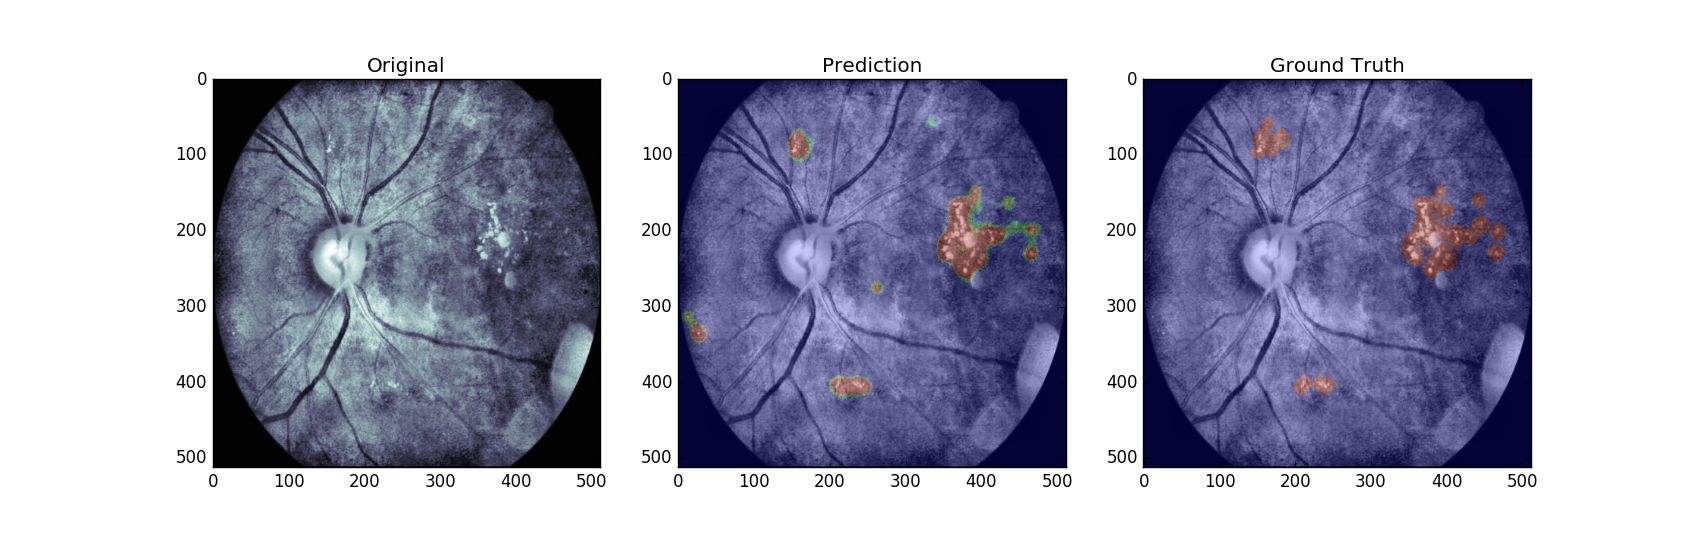
\includegraphics{C:/Users/yidar/Desktop/candle/reports/figures/EX-seg/C0021834.h5.png}
\caption{}
\end{figure}

\begin{figure}
\centering
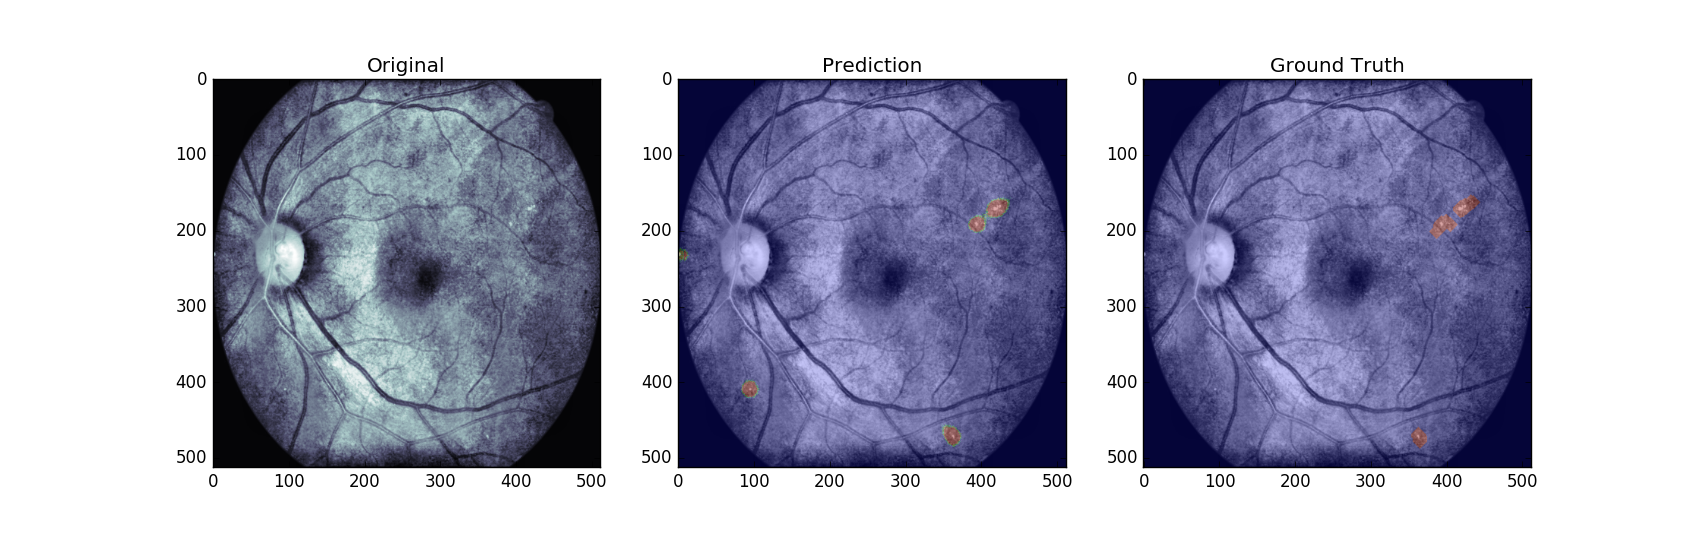
\includegraphics{C:/Users/yidar/Desktop/candle/reports/figures/EX-seg/C0021835.h5.png}
\caption{}
\end{figure}

\begin{figure}
\centering
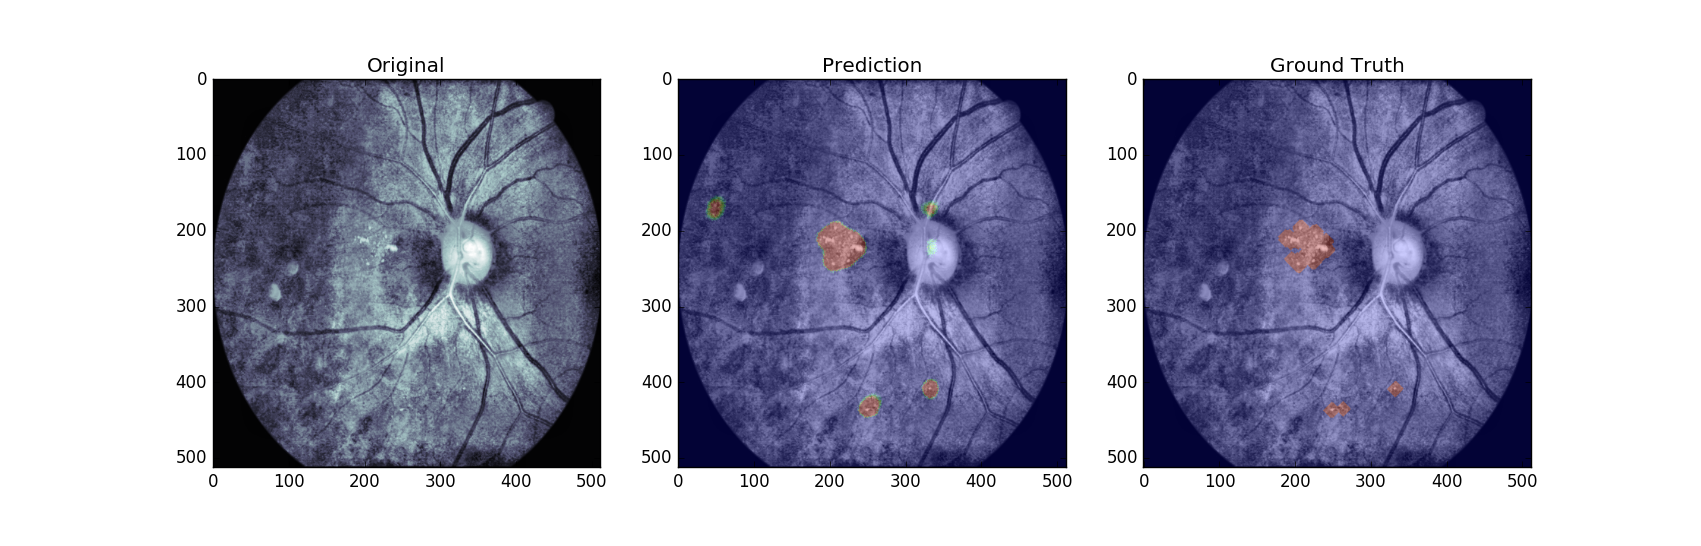
\includegraphics{C:/Users/yidar/Desktop/candle/reports/figures/EX-seg/C0021836.h5.png}
\caption{}
\end{figure}

\begin{figure}
\centering
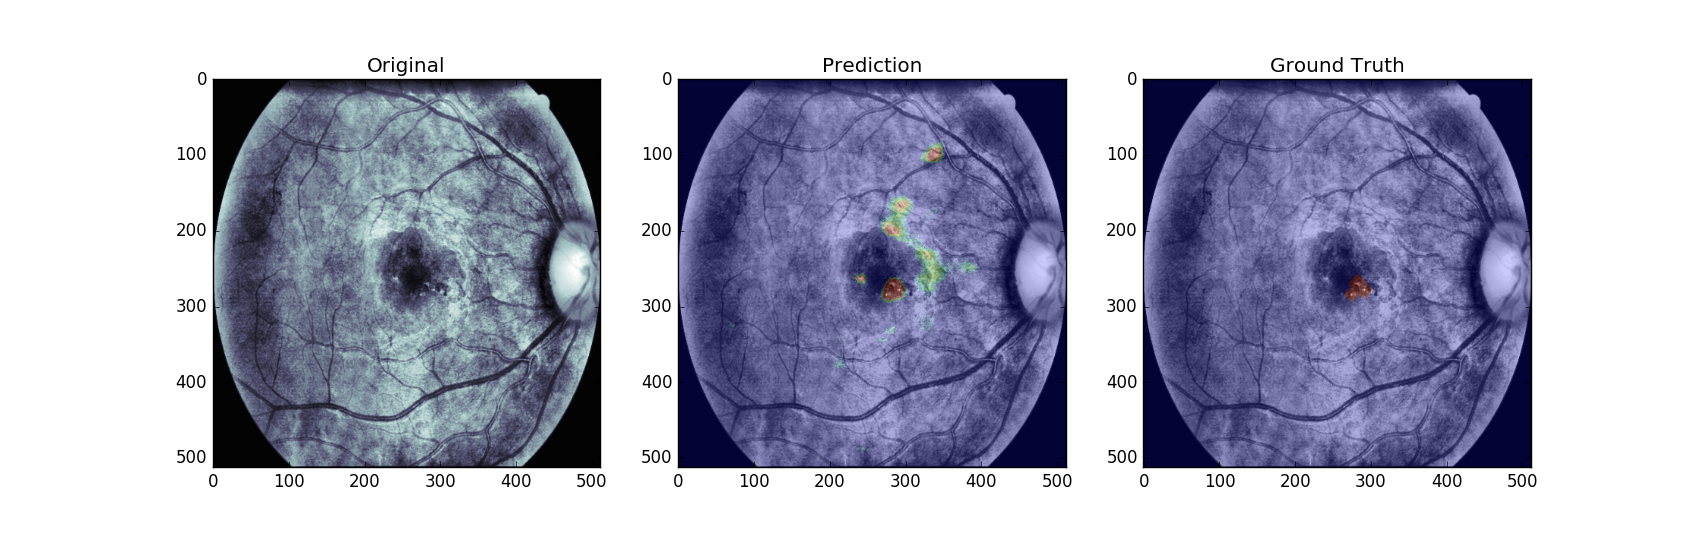
\includegraphics{C:/Users/yidar/Desktop/candle/reports/figures/EX-seg/C0025307.h5.png}
\caption{}
\end{figure}

\begin{figure}
\centering
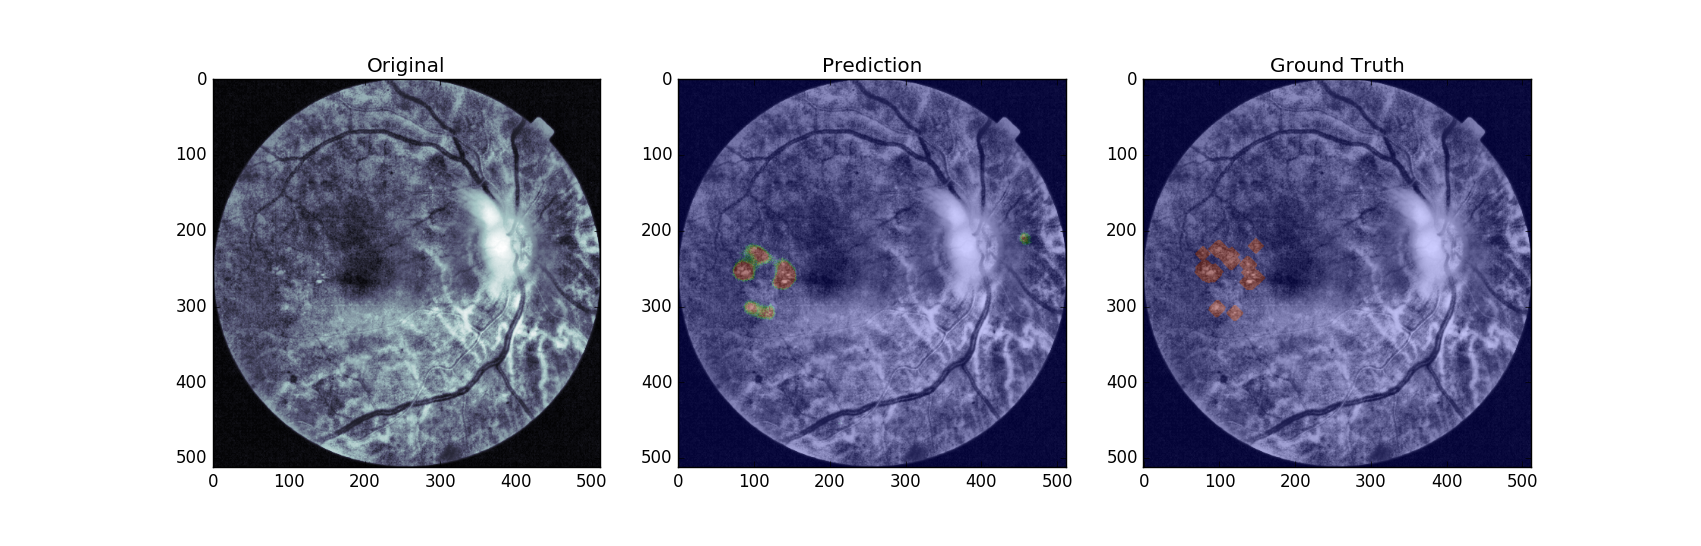
\includegraphics{C:/Users/yidar/Desktop/candle/reports/figures/EX-seg/DS000OTS.h5.png}
\caption{}
\end{figure}

\clearpage
\clearpage
\clearpage
\pagebreak

    \subsubsection{Microaneurisms}\label{microaneurisms}

These were a bit trickier. To be honest, the exudates will train even
without the histogram normalization. The microaneurisms will not train
without the adaptive histogram equalization. They also take about twice
the time to train as the exudates. This is because the features are MUCH
MUCH smaller.

However, after training all the high contrast images for more than an
hour (50+ epochs), we do see some results.

\begin{figure}
\centering
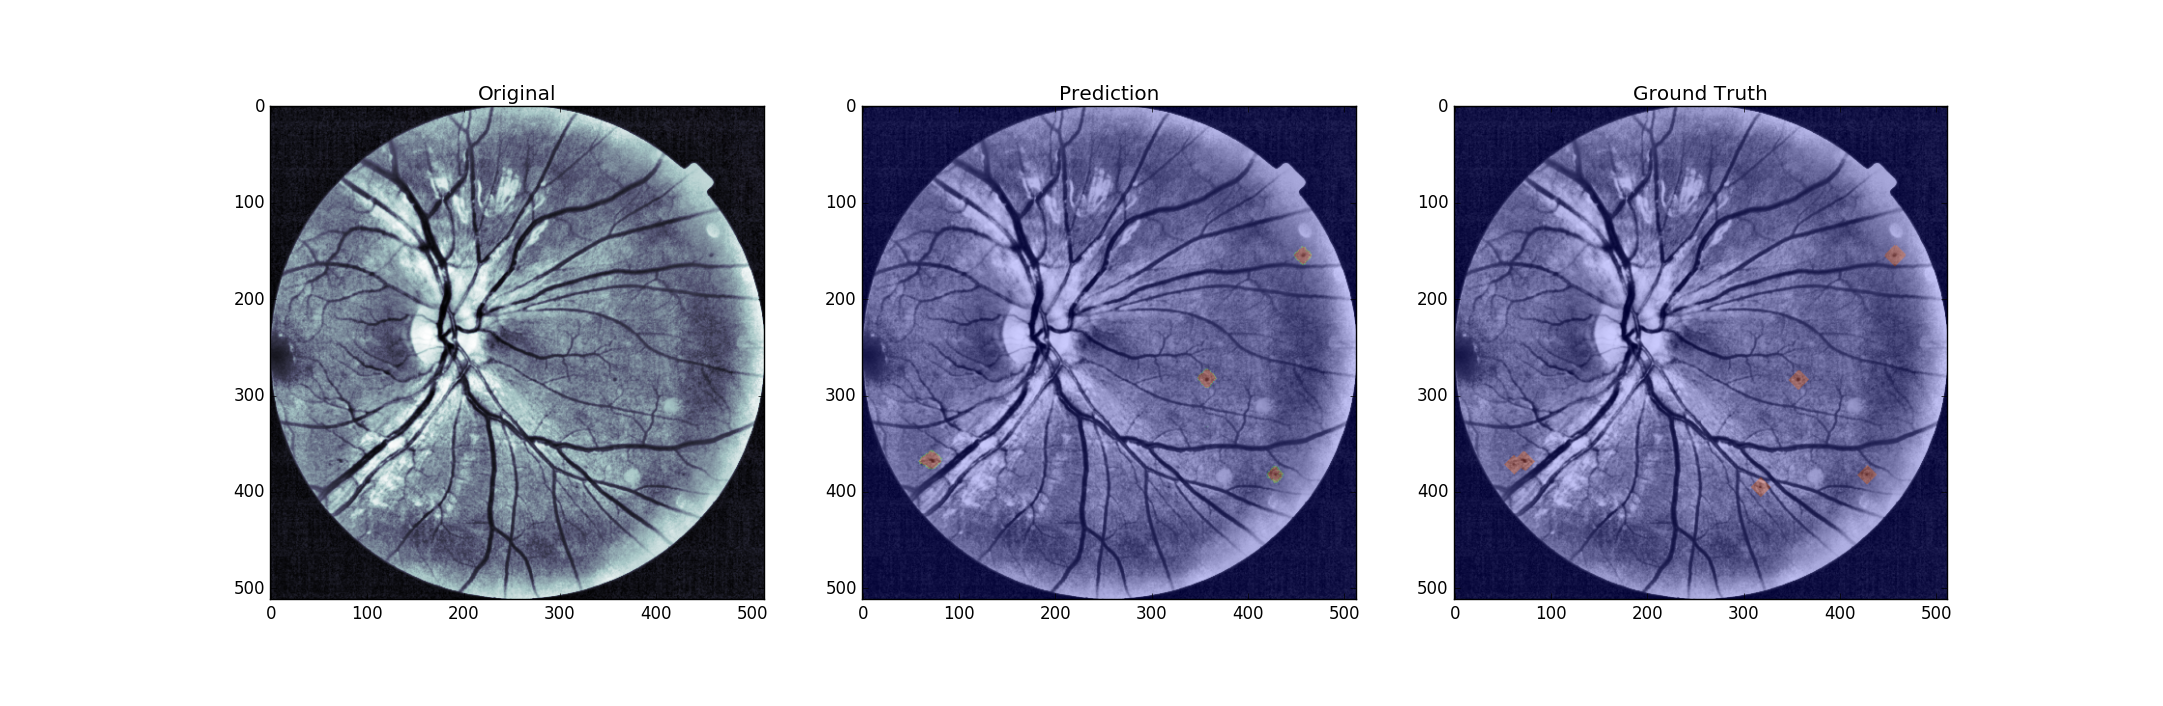
\includegraphics{C:/Users/yidar/Desktop/candle/reports/figures/MA-seg/DS000DBP.h5.png}
\caption{}
\end{figure}

\begin{figure}
\centering
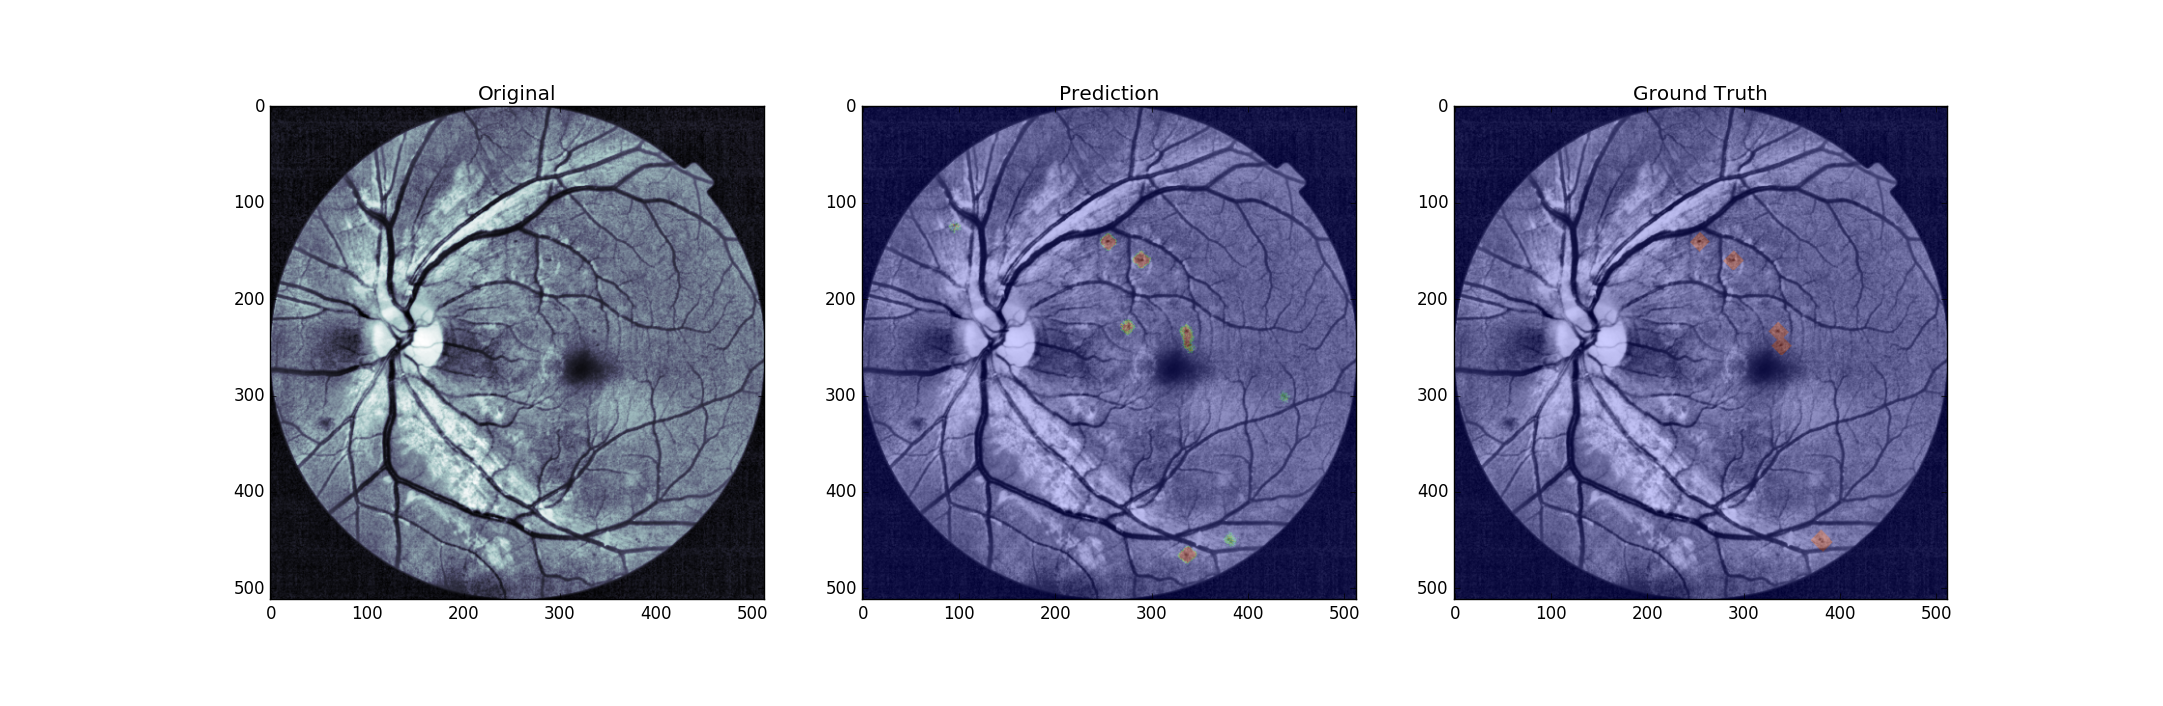
\includegraphics{C:/Users/yidar/Desktop/candle/reports/figures/MA-seg/DS000DBQ.h5.png}
\caption{}
\end{figure}

\begin{figure}
\centering
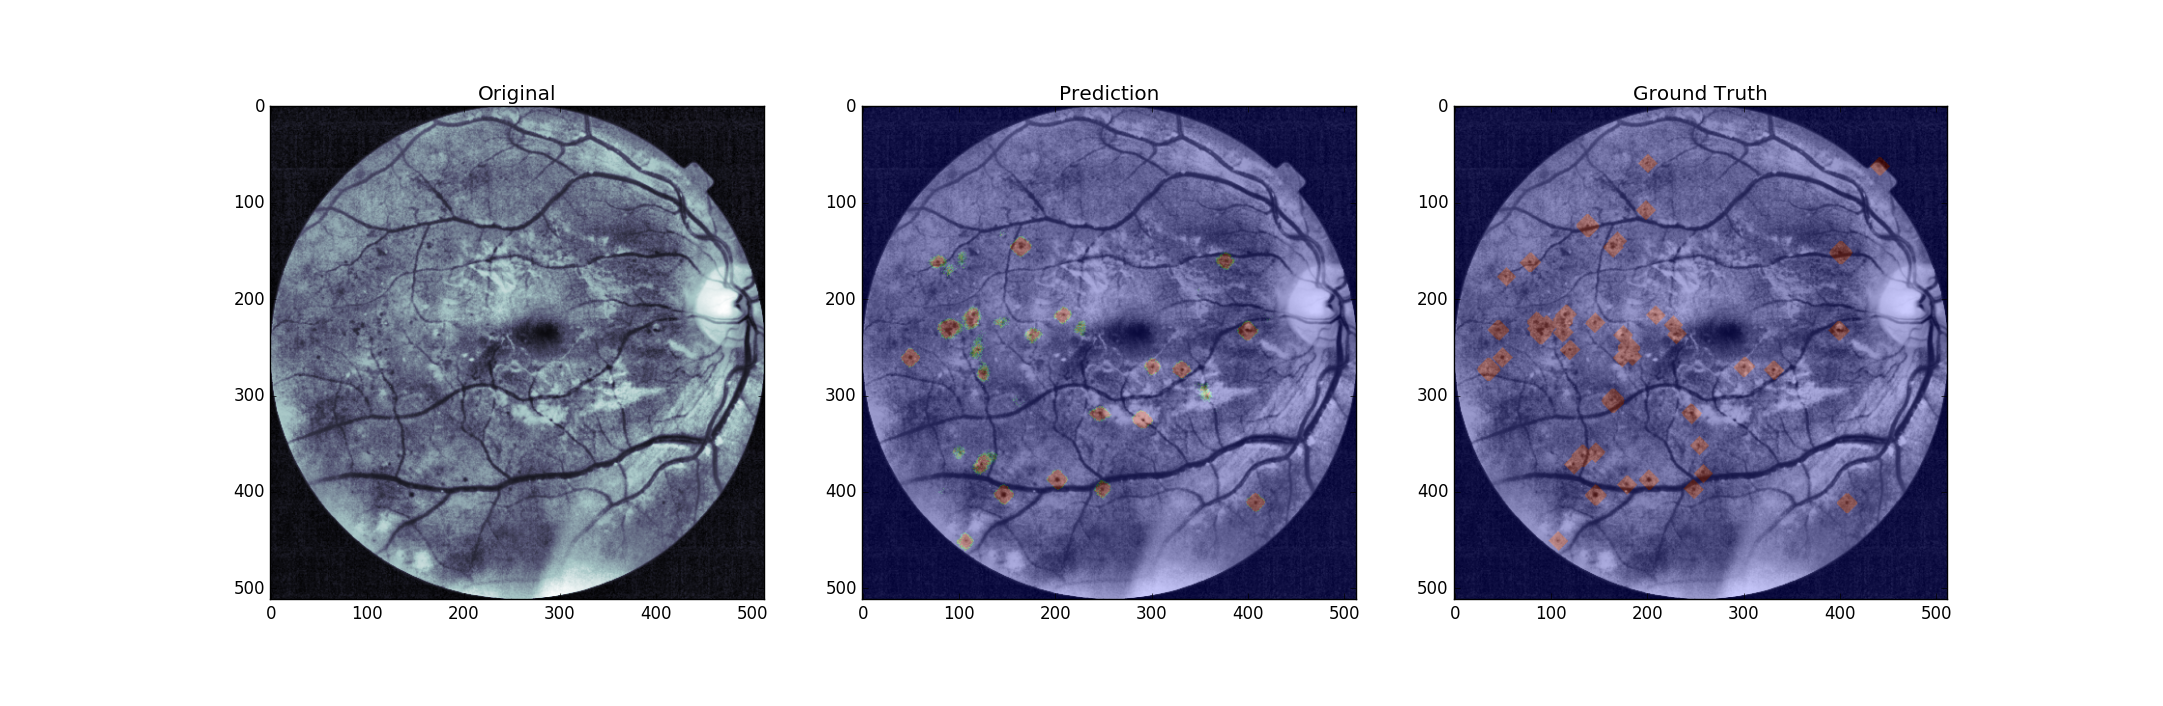
\includegraphics{C:/Users/yidar/Desktop/candle/reports/figures/MA-seg/DS000DPJ.h5.png}
\caption{}
\end{figure}

\begin{figure}
\centering
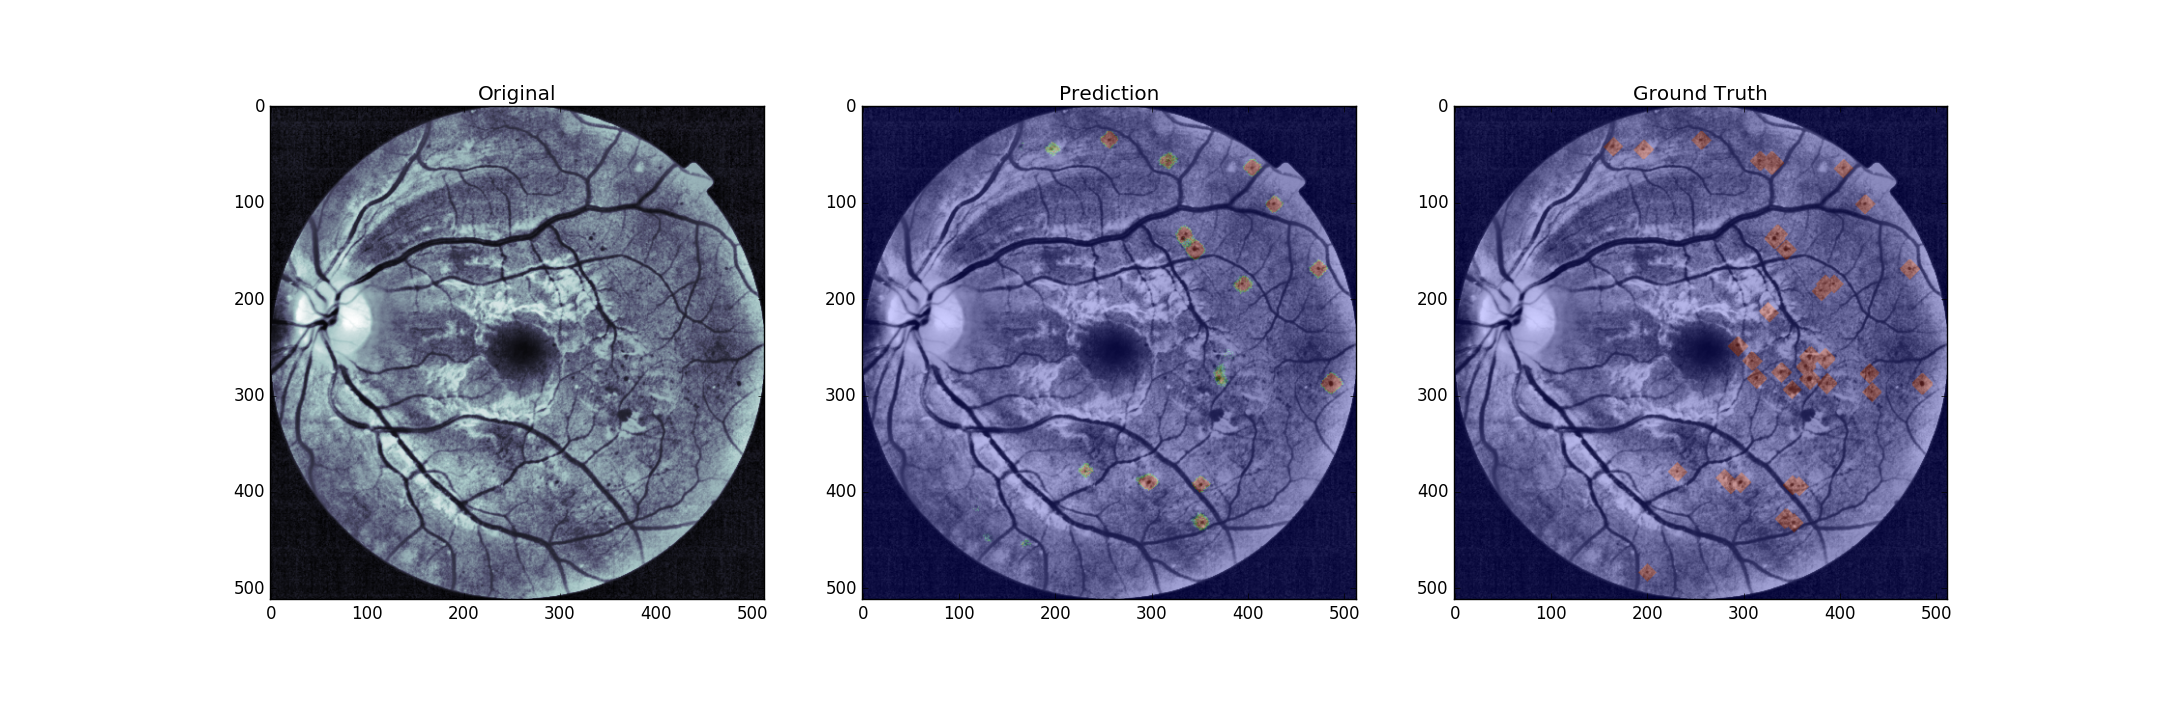
\includegraphics{C:/Users/yidar/Desktop/candle/reports/figures/MA-seg/DS000DPL.h5.png}
\caption{}
\end{figure}

\begin{figure}
\centering
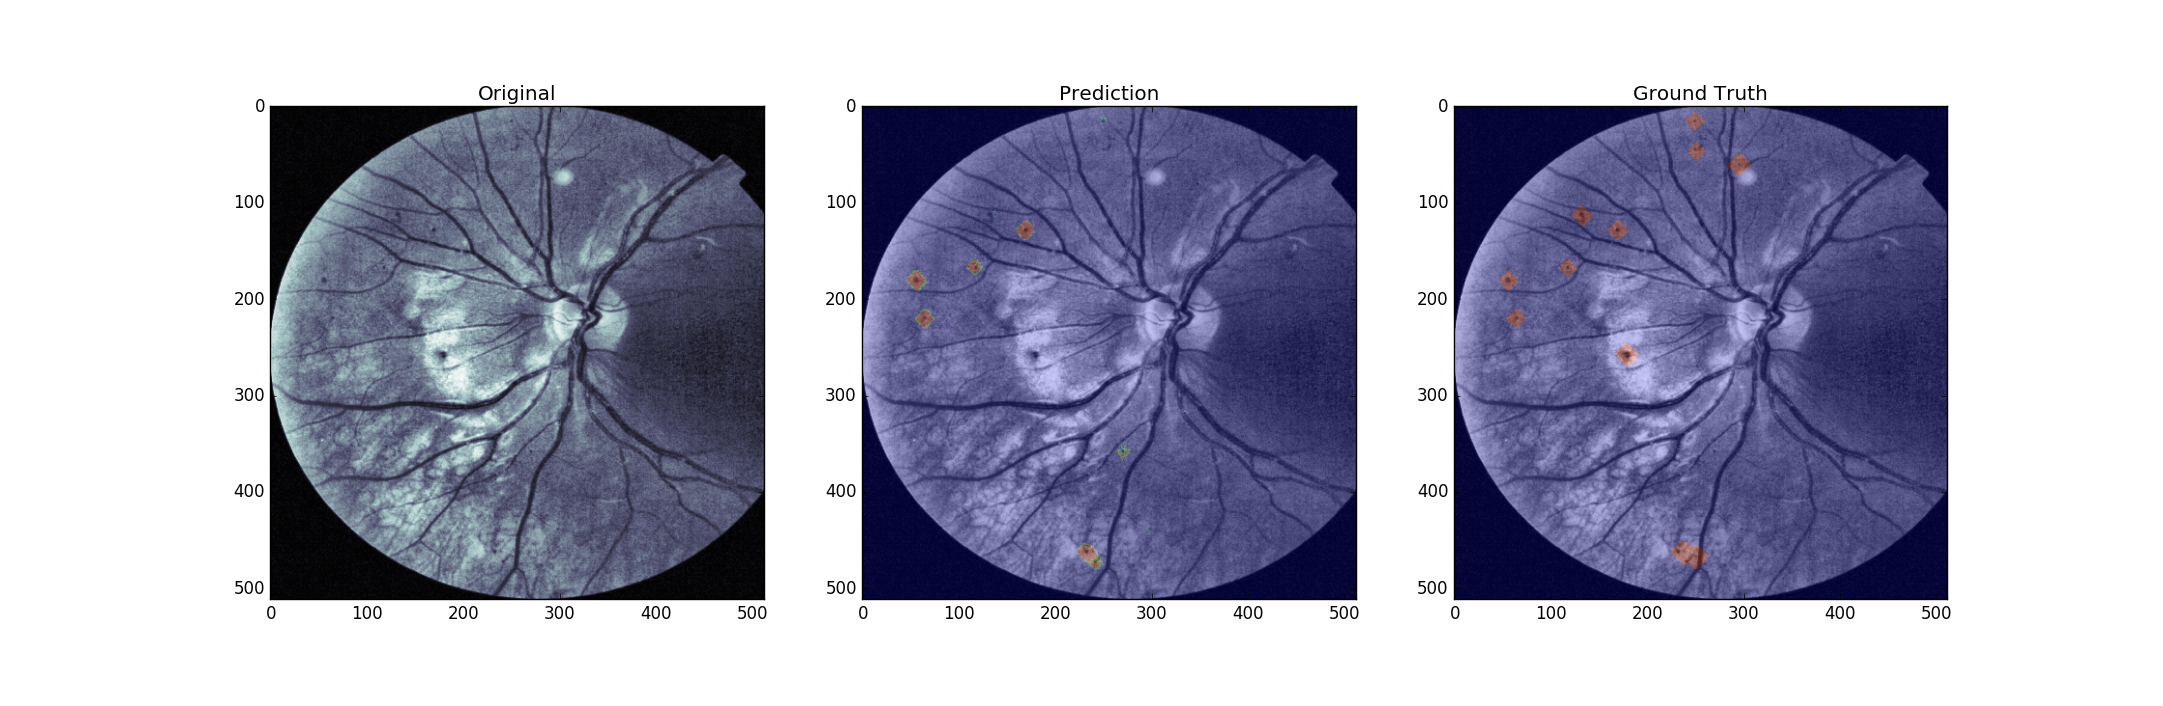
\includegraphics{C:/Users/yidar/Desktop/candle/reports/figures/MA-seg/DS000NA1.h5.png}
\caption{}
\end{figure}

    \subsection{Diabetic Retinopathy
Challenge}\label{diabetic-retinopathy-challenge}

For the preliminary results, we simply separated a training and
validation set. We applied the preprocessing steps as stated above
(cropping and adaptive histogram equalization).

The data has the following splits: - Label 0: Normals - 73.48\% - Label
1: Mild DR - 6.96\% - Label 2: Moderate DR - 15.07\% - Label 3: Sever DR
- 2.48\% - Label 4: Proliferative DR - 2.01\%

Thus, we should be seeing a majority classifier of about 73.5\%. We
don't do much better, but we do indeed do better than the majority
classifer. If we're being generous, we have a validation accuracy of
about 85\%, a 10\% increase on the majority classifier.

\begin{figure}
\centering
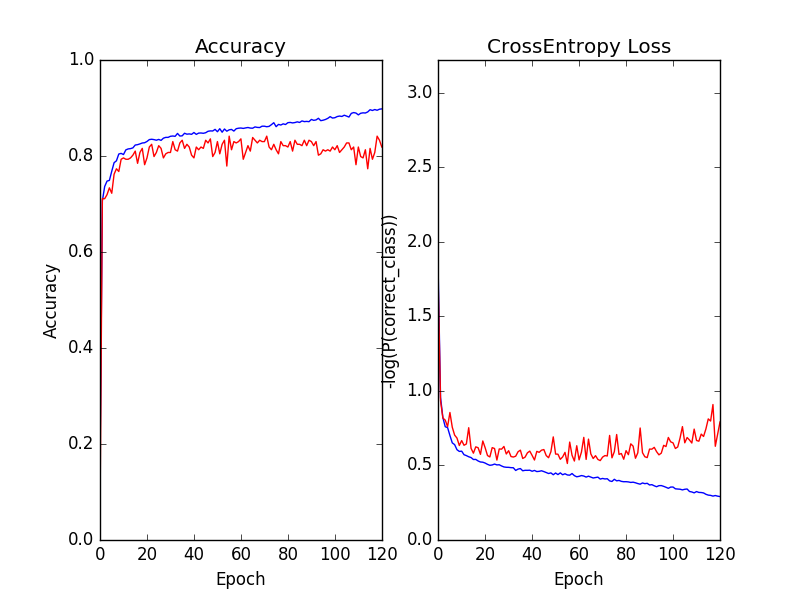
\includegraphics{C:/Users/yidar/Desktop/candle/reports/figures/DR_kaggle/DR_kaggle.png}
\caption{}
\end{figure}

    \begin{Verbatim}[commandchars=\\\{\}]
{\color{incolor}In [{\color{incolor} }]:} 
\end{Verbatim}


    % Add a bibliography block to the postdoc
    
    
    
    \end{document}
